\section{STM in ABS}
\label{sec:stm_abs}
In this section we give a short overview of how to apply STM in ABS. We fundamentally follow a time-driven approach in both case studies where the simulation is advanced by some given $\Delta t$ and in each step all agents are executed. To employ parallelism, each agent runs within its own thread and agents are executed in lock-step, synchronising between each $\Delta t$ which is controlled by the main thread. This way of stepping the simulation is introduced in \cite{thaler_art_2017} on a conceptual level, where the authors name it \textit{concurrent update-strategy}. See Figure \ref{fig:stm_abs_structure} for a visualisation of our concurrent, time-driven lock-step approach. 

An agent thread will block until the main thread sends the next $\Delta t$ and runs the \texttt{STM} action atomically with the given $\Delta t$. When the \texttt{STM} action has been committed, the thread will send the output of the agent action to the main thread to signal it has finished. The main thread awaits the results of all agents to collect them for output of the current step e.g. visualisation or writing to a file.

As will be described in subsequent sections, central to both case studies is an environment which is shared between the agents using a \texttt{TVar} or \texttt{TArray} primitive through which the agents communicate concurrently with each other. To get the environment in each step for visualisation purposes, the main thread can access the \texttt{TVar} and \texttt{TArray} as well. 

\begin{figure}
	\centering
	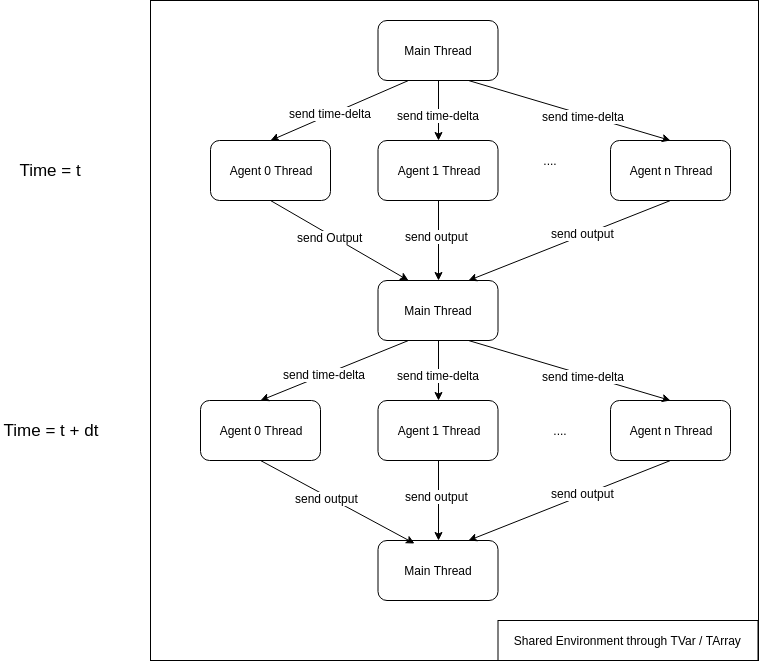
\includegraphics[width=0.6\textwidth, angle=0]{./fig/dia/stm_abs.png}
	\caption{Diagram of the parallel time-driven lock-step approach.}
	\label{fig:stm_abs_structure}
\end{figure}

\subsection{Adding STM to agents}
We briefly discuss how to add STM to agents on a technical level and also show how to run them within their own threads. We use the SIR implementation as example - applying it to the Sugarscape implementation works exactly the same way.

TODO: refer to my pure FP paper, as it is beyond the focus of this paper

The first step is to simply add the \texttt{STM} Monad as the innermost level to the already the existing Transformer stack. Further, the environment is now passed as a transactional data primitive to the agent at \textit{construction time}. Thus, the agent does not receive the \texttt{SIREnv} as input any more but receives it through currying when constructing its initial \texttt{MSF}. Further, the agent modifies the \texttt{SIREnv} directly through the \texttt{TVar}, as demonstrated in the case of the infected agent.

\begin{HaskellCode}
-- Make Rand a transformer to be able to add STM as innermost monad
type SIRMonad g = RandT g STM
-- Input to agent is now an empty tuple instead of the Environment
type SIRAgent g = SF (SIRMonad g) () SIRState

-- The MSF construction function takes now the TVar with the environment.
sirAgent :: RandomGen g => TVar SIREnv -> Disc2dCoord -> SIRState -> SIRAgent g

-- The infected agent behaviour is nearly the same except that
-- the agent modifies the environment through the TVar
infected :: RandomGen g => SF (SIRMonad g) () (SIRState, Event ())
infected = proc _ -> do
  recovered <- occasionally illnessDuration () -< ()
  if isEvent recovered
    then (do
      -- update the environment through the TVar
      arrM_ (lift $ lift $ modifyTVar env (changeCell coord Recovered)) -< ()
      returnA -< (Recovered, Event ()))
    else returnA -< (Infected, NoEvent)
\end{HaskellCode}

The agent thread is straightforward. It takes \texttt{MVar} synchronisation primitives to synchronise with the main thread and simply runs the agent behaviour each time it receives the next \textit{DTime}:

\begin{HaskellCode}
agentThread :: RandomGen g 
            => Int             -- ^ Number of steps to compute
            -> SIRAgent g      -- ^ Agent behaviour MSF
            -> g               -- ^ Random-number generator of the agent
            -> MVar SIRState   -- ^ Synchronisation back to main thread
            -> MVar DTime      -- ^ Receiving DTime for next step
            -> IO ()
agentThread 0 _ _ _ _ = return () -- all steps computed, terminate thread
agentThread n sf rng retVar dtVar = do
  -- wait for dt to compute current step
  dt <- takeMVar dtVar

  -- compute output of current step
  let sfReader = unMSF sf ()
      sfRand   = runReaderT sfReader dt
      sfSTM    = runRandT sfRand rng
  -- run the STM action atomically within IO
  ((ret, sf'), rng') <- atomically sfSTM 

  -- post result to main thread
  putMVar retVar ret
  
  -- tail recursion to next step 
  agentThread (n - 1) sf' rng retVar dtVar
\end{HaskellCode}

Computing a simulation step is now trivial within the main thread. All agent threads \texttt{MVars} are signalled to unblock followed by an immediate block on the \texttt{MVars} into which the agent threads post back their result. The state of the current step is then extracted from the environment, which is stored within the \texttt{TVar} which the agent threads have updated.

\begin{HaskellCode}
simulationStep :: TVar SIREnv     -- ^ environment 
               -> [MVar DTime]    -- ^ sync dt to threads
               -> [MVar SIRState] -- ^ sync output from threads
               -> DTime           -- ^ time delta
               -> IO SIREnv
simulationStep env dtVars retVars dt = do
  -- tell all threads to continue with the corresponding DTime
  mapM_ (`putMVar` dt) dtVars
  -- wait for results but ignore them, SIREnv contains all states
  mapM_ takeMVar retVars
  -- return state of environment when step has finished
  readTVarIO env
\end{HaskellCode}